\chapter{Overzicht werking}\label{hs:werking}

\section{Algemeen}
Gebruik Java/Perl/... uitleggen

\section{WEKA}
WEKA (Waikato Environment for Knowledge Analysis) is een tool voor datamining ontwikkeld in de programmeertaal Java. Het bestaat uit een grafische werkomgeving  voor het uitvoeren van de nodige stappen bij datamining, een CLI en is volledig ondersteund voor gebruik binnen een eigen Java-programma. Het helpt bij de preprocessing van data en bevat heel wat algoritmes voor clustering, classificatie, regressie-analyse, visualisatie en feature selection.

De versie van WEKA die gebruikt wordt in deze masterproef is 3.6.13, de op heden laatste stabiele versie.

\textbf{TODO: meer + referentie}

\section{Voorbereiden van de dataset}
\subsection{Verwerking met Apache Tika}
Om met verschillende documentencollecties te kunnen werken binnen het ontworpen systeem, wordt gebruik gemaakt van Apache Tika \cite{tika}. Tika laat toe om metadata van een tekst af te leiden. Die metadata kan o.a. de taal of het formaat van het document in kwestie zijn. Deze data kan belangrijk zijn bij de keuze van het stemmingsalgoritme dat gebruikt moet worden (dit is afhankelijk van de taal, zie \ref{stemming}) of laat toe om verschillende soorten documentformaten (pdf, doc, docx, csv, html, etc) om te vormen tot platte tekst zonder franjes. Deze tekst kan veel beter ge\"interpreteerd worden door een computer.
Apache tika wordt aangeboden onder de vorm van een REST-API, gebouwd op het Jersey-framework in Java. Het Jersey-framework is gebaseerd op JAX-RS en laat toe om verschillende types data aan te bieden aan de gebruiker. Het wordt gedeployed naar een Glassfish-omgeving, die vervolgens kan worden aangesproken door gebruikers van de API.

Op zich bevat de API slechts twee verschillende \textit{endpoints}; \quotes{/test} controleert of de API wel degelijk reageert op calls, terwijl \quotes{/upload} een document aanvaardt in de vorm van een tekst en die gaat parsen naar platte tekst. Het parsen bestaat uit twee delen. Het eerste deel is de taaldetectie, welke door de standaard \textit{LanguageIdentifier} van het Tika framework wordt uitgevoerd. Het tweede deel vervolgens is het effectief parsen van de tekst. Hiervoor wordt de \textit{AutoDetectParser} van Tika gebruikt. Deze kiest voor elk document de parser die voor dat type het beste resultaat zal opleveren.
De resultaten van de parser worden teruggestuurd naar de initiator van de connectie in de vorm van JSON:

\begin{lstlisting}
{
"language":"nl",
"title":"5-000-deelnemers-opname-clip-klimaatsverandering\n",
"body":"Op het Klein Strand in Oostende zijn vanmiddag naar schatting 5.000 mensen samengekomen op een klimaathappening die onderdeel was van de internationale campagne 'The Big Ask'. De deelnemers figureerden in een filmpje van regisseur Nic Baltazar en Friends of the Earth vzw.Filmpje YoutubeOp het Klein Strand vormden de deelnemers letters en slogans die vanuit de hoogte werden opgenomen en later zullen te zien zijn in een filmpje op Youtube. De actie 'Sos Klimaat : bouw een dijk tegen klimaatsverandering' kreeg de steun van talrijke BV's die als dj de massa animeerden. Onder meer Zohra, Flip Kowlier, Gabriel Rios en Adriaan Van den Hoof verleenden op het podium hun medewerking.Politici wakkerschuddenInitiatiefnemer Nic Baltazar was in elk geval tevreden met de opkomst en de opnames en verwacht dat de clip op Youtube voor een half miljoen hits zal zorgen. Hij hoopt dat de actie en de clip politici zal wakker schudden omtrent de problematiek. (belga/ep)\n"
}
\end{lstlisting} 

\subsection{Preprocessing van tekstdocumenten}\label{bag-of-words}
De platte tekst in de documentencollectie bevat op zich te weinig structuur om effici\"ent verwerkt te worden door een computer. Om de data beter te kunnen begrijpen moeten we de dataset eerst omvormen tot een feature vector die vervolgens als input kan dienen voor content recognition systemen. Omdat de noden voor zowel classificatie en clustering niet volledig dezelfde zijn, worden ze telkens opgesplits en waar nodig verduidelijkt.

\subsubsection{Tokenization}
Om alle woorden te verkrijgen die gebruikt worden in een bepaalde tekst, wordt een \textit{tokenization}\label{tokenization} proces toegepast. Dit zorgt ervoor dat een tekstdocument gesplitst wordt in een stroom van woorden door alle leestekens te verwijderen en alle tabs en niet-tekstuele karakters door spaties te vervangen. De set van verschillende woorden uit alle tekstdocumenten wordt samengevoegd tot het woordenboek van de documentencollectie. 

Het is echter ook mogelijk om een N-Gram tokenizer \cite{McNamee2004} te gebruiken. Deze geeft de mogelijkheid om eventueel twee of drie woorden samen te nemen en die als \'e\'en woord in onze documentencollectie te zien. Dit kan voordeel geven bij o.a. personennamen, welke vaak bestaan uit twee woorden die voor een tekst belangrijk zouden kunnen zijn. Uiteraard wordt een eigennaam ook opgepikt indien alle woorden apart beschouwd worden.

Om de grootte van het woordenboek en dus de dimensionaliteit van de beschrijving van de documentencollectie te verkleinen, wordt de set van woorden verder gereduceerd door het toepassen van filters of \textit{stemming}salgoritmes. 

\subsubsection{Filter- en stemmingsalgoritmes}\label{stemming}
Filters verwijderen woorden van het woordenboek en dus uit de documenten. De filtering die het meest wordt toegepast op tekstuele collecties is stopwoordfiltering. De stopwoorden die verwijderd worden zijn woorden die weinig of geen inhoud hebben. Voorbeelden zijn lidwoorden, verbindingswoorden, voorzetsels, etc. \\
Stemmingsalgoritmes proberen een woord om te vormen tot de standaardvorm van dat woord. Dit doen ze bijvoorbeeld door meervouden van zelfstandige naamwoorden naar het enkelvoud om te zetten of door werkwoorden naar hun stam te vereenvoudigen. Het stemmingalgoritme dat hier gebruikt wordt is Porters stemming algoritme voor de Nederlandse taal \cite{Kraaij1994}. Het is een implementatie van Porters stemming algoritme \cite{Porter1980}, dat origineel enkel voor de Engelse taal werd ontworpen.

\subsection{Vector space model}\label{vector-space-model}
Ondanks de simpele datastructuur zorgt het vector space model ervoor dat grote collecties documenten effici\"ent kunnen geanalyseerd worden. Het representeert documenten als vectors in een $m$-dimensionale ruimte. Elk document $d$ uit de documentencollectie is beschreven als een numerieke\textit{ feature vector} $w(d) = (x(d,t_1),...,x(d,t_m))$ waarbij $T=\{t_1,...,t_m\}$ het woordenboek voorstelt. De hoofdtaak van de vector space representatie van documenten is het vinden van een geschikte encodering van de feature vector. 

Elk element van de vector representeert meestal een woord (of groep van woorden) van de documentencollectie. De simpelste manier om een document te encoderen is om \textit{binary term} vectoren te gebruiken. Als een woord voorkomt in het document wordt het corresponderende element op \'e\'en gezet, komt het niet voor dan is het nul. De encodering wordt zo herleid tot een simpele Booleaanse vergelijking. Hierbij wordt de belangrijkheid van elk woord als gelijkwaardig beschouwd. 

Om de performantie te verbeteren kunnen \textit{term weighting schemes} worden gebruikt \cite{Salton1988}. Het gewicht dat toegekend wordt aan een woord reflecteert de belangrijkheid of relevantie van dat woord in een specifiek document of collectie. Een woord met hoge frequentie in bepaalde documenten, maar dat weinig of niet voorkomt in de volledige documentencollectie wordt een groot gewicht toebedeeld. Een gewicht $w(d,t)$ voor term $t$ in document $d$ wordt berekend als de term frequency $tf(d,t)$ vermenigvuldigd met de inverse document frequency $idf(t)$ - gedefinieerd als $idf(t)=\log{\frac{N}{n_t}})$. Dit beschrijft de specifiteit van een bepaalde term in een documentencollectie. 

Naast term frequency en inverse document frequency wordt een normalisatie toegepast om ervoor te zorgen dat alle documenten dezelfde kans hebben om gevonden te worden, onafhankelijk van hun lengte. Deze techniek heeft zijn nut reeds bewezen in de praktijk . 
\begin{equation}\label{eq:tfidf}
w(d,t) = \frac{tf(dt)\log{\frac{N}{N_t}}}{\sqrt{\sum_{j=1}^{m}tf(d,t_j)^2(log(\frac{N}{n_{t_j}}))^2}}
\end{equation}
Hierbij stelt $N$ de grootte van de documentencollectie $D$ voor en is $n_t$ het aantal documenten in $D$ dat term $t$ bevat.

\subsection{Feature selection}
Feature selection of attribute selection zorgt ervoor dat attributen die niet relevant zijn verwijderd worden. Zo wordt een subset van de features gezocht die relevant zijn voor het doelconcept. Dit zorgt er o.a. voor dat de dataset kleiner wordt, waardoor minder rekenkracht en zoekruimte vereist is bij de effectieve verwerking van het vector model. Volgens \cite{Liu2005} is het \'e\'en van de meest belangrijke en meest gebruikte technieken voor data preprocessing bij data mining. Het reduceert het aantal features, het verwijdert irrelevante of redundante data en het zorgt er bijgevolg voor dat data mining algoritmes sneller werken. Het zorgt er o.m. ook voor dat de voorspelde accuraatheid en begrijpbaarheid van de resultaten verbeterd wordt. Feature selection is vooral interessant bij text mining, omdat er een hoge dimensionaliteit is van de features en er veel irrelevante features voorkomen.

Als de dimensionaliteit van een domein bovendien vergroot wordt, verhoogt het aantal features $N$. Een optimale subset van features vinden is zeer moeilijk en veel problemen gerelateerd aan feature selection zijn NP-moeilijk. Volgens \cite{Liu2005} bestaat een typisch feature selection proces uit vier stappen (zie figuur \ref{fig:feature-selection}); subset generatie, subset evaluatie, stopcriterium en resultatenvalidatie.

\begin{figure}[h]
	\caption{Vier stappen in feature selection}
	\label{fig:feature-selection}
	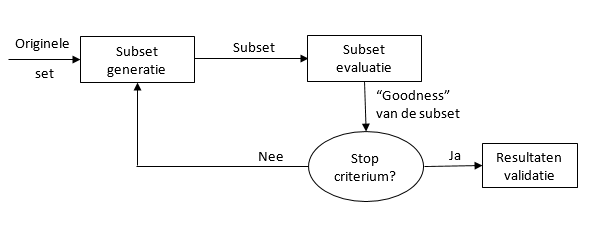
\includegraphics[width=\textwidth]{fig/feature-selection}
\end{figure}

Subset generatie is een zoekprocedure die kandidaat feature subsets produceert voor evaluatie met een bepaalde zoekstrategie. Elke kandidaat subset wordt ge\"evalueerd en vergeleken met de vorige beste volgens een bepaald criterium. Als de nieuwe subset beter is, wordt de vorige beste subset vervangen. Dit proces wordt herhaald tot een bepaald stopcriterium is bereikt. Dan wordt de geselecteerde beste subset gevalideerd met voorkennis of via verschillende tests op andere datasets. Feature selection is zowel interessant voor classificatie als clustering. 

\section{Classificatie}
Een eerste techniek die toegepast wordt om een aanbevelingssysteem een beter beeld te geven van de documentencollectie, is classificatie. Door een artikel automatisch aan een categorie te kunnen toewijzen, krijgen we al een veel duidelijker beeld van waarover dit artikel nu precies handelt. Als we zowel de hoofd- als subcategorie van een artikel kunnen bepalen, hebben we al een eerste sterke indicatie of het artikel al dan niet interessant kan zijn voor de gebruiker en dus aanbevolen zal worden door het aanbevelingssysteem. 

WEKA ondersteunt echter slechts \'e\'en niveau van classificatie. Om dit probleem op te lossen gaan we eerst de artikels indelen in de hoofdcategorie\"en en pas daarna in de subcategorie\"en. Omdat het mogelijk is dat voor deze gevallen een andere classifier en een ander aantal woorden optimaal is, gaan we deze apart testen. De preprocessing blijft voor alle gevallen gelijk. Wel gaan we eerst uitzoeken welke parameters van de preprocessing het beste beeld geven voor enkele na\"ieve classifiers. 

\subsection{Parameters voor preprocessing van data}

Om de optimale parameters voor de preprocessing te bepalen wordt een classificatie uitgevoerd met de verwerkte dataset. We vari\"eren de parameters en bepalen zo de optimale instellingen. De dataset die eerst gebruikt wordt is deze van Het Laatste Nieuws, januari 2008. De classifiers die gebruikt worden om de bekomen woordvector te testen zijn "Naive Bayes$"$ en "Naive Bayes Multinomial". 

Om een betrouwbaar resultaat te bekomen worden de tests met een \textit{10-fold cross validation}\label{10-fold-cv} uitgevoerd. Dit is een techniek om voorspellende modellen te evalueren door de originele dataset te verdelen in een trainingsset om het model te trainen en een testset om deze te valideren. Bij 10-fold cross-validation\label{cross-val} wordt de originele dataset random verdeeld in 10 subsets. Daarvan wordt \'e\'en subset behouden ter validatie van het model. De overige 9 subsets worden gebruikt als trainingsdata. Het cross-validation proces wordt 10 keer herhaald, waarbij elk van de subsets exact \'e\'en keer gebruikt worden als validatieset. De 10 resultaten worden gecombineerd (uitgemiddeld) om een enkele voorspelling te maken. Het grote voordeel van deze methode is dat alle observaties zowel gebruikt worden als trainings- en validatiedata. 

Om de resultaten onafhankelijk te stellen van het aantal woorden dat behouden wordt van de documentencollectie, gebruiken we de standaard bijgehouden 1000 woorden. Verder worden de verschillende parameters al dan niet ingesteld, zoals te zien in tabel \ref{tab:preprocessing-params}. Hierbij staat \quotes{1} voor gebruikt en \quotes{0} voor niet gebruikt. 

\begin{longtable}{rrrrrrr}
	\caption{Gebruik van verschillende parameters bij preprocessing van de documentencollectie en hun effect op het percentage correct geclassificeerde artikels volgens de "Naive Bayes$"$ (NB) en "Naive Bayes Multinomial" (NBM) classifiers.}\\
	\toprule
	\multicolumn{1}{c}{\textbf{tf-idf}} & \multicolumn{1}{c}{\textbf{Stemming}} & \multicolumn{1}{c}{\textbf{Stopwoorden}} & \multicolumn{1}{c}{\textbf{Frequentie}} & \multicolumn{1}{c}{\textbf{Tokenizer}} & \multicolumn{1}{c}{\textbf{NB}} & \multicolumn{1}{c}{\textbf{NBM}} \\
	\midrule
	0     & 0     & 0     & 0     & 1     & 69.85\% & 74.39\% \\
	0     & 0     & 0     & 0     & 2     & 67.62\% & 72.34\% \\
	0     & 0     & 0     & 0     & 3     & 67.44\% & 72.15\% \\
	0     & 0     & 0     & 1     & 1     & 56.06\% & 66.39\% \\
	0     & 0     & 0     & 1     & 2     & 54.26\% & 64.35\% \\
	0     & 0     & 0     & 1     & 3     & 54.24\% & 64.30\% \\
	0     & 0     & 1     & 0     & 1     & 71.50\% & 75.71\% \\
	0     & 0     & 1     & 0     & 2     & 69.26\% & 73.41\% \\
	0     & 0     & 1     & 0     & 3     & 68.91\% & 73.09\% \\
	0     & 0     & 1     & 1     & 1     & 58.01\% & 68.31\% \\
	0     & 0     & 1     & 1     & 2     & 56.25\% & 66.18\% \\
	0     & 0     & 1     & 1     & 3     & 56.20\% & 66.09\% \\
	0     & 1     & 0     & 0     & 1     & 70.85\% & 75.43\% \\
	0     & 1     & 0     & 0     & 2     & 68.19\% & 72.65\% \\
	0     & 1     & 0     & 0     & 3     & 68.35\% & 72.61\% \\
	0     & 1     & 0     & 1     & 1     & 57.68\% & 67.55\% \\
	0     & 1     & 0     & 1     & 2     & 55.74\% & 65.36\% \\
	0     & 1     & 0     & 1     & 3     & 55.88\% & 65.43\% \\
	0     & 1     & 1     & 0     & 1     & \textbf{71.91\%} & \textbf{76.37\%} \\
	0     & 1     & 1     & 0     & 2     & 69.44\% & 73.82\% \\
	0     & 1     & 1     & 0     & 3     & 69.42\% & 73.70\% \\
	0     & 1     & 1     & 1     & 1     & 59.09\% & 69.31\% \\
	0     & 1     & 1     & 1     & 2     & 57.49\% & 67.30\% \\
	0     & 1     & 1     & 1     & 3     & 57.29\% & 67.07\% \\
	1     & 0     & 0     & 0     & 1     & 36.40\% & 57.44\% \\
	1     & 0     & 0     & 0     & 2     & 40.78\% & 58.42\% \\
	1     & 0     & 0     & 0     & 3     & 40.85\% & 58.31\% \\
	1     & 0     & 0     & 1     & 1     & 40.88\% & 59.59\% \\
	1     & 0     & 0     & 1     & 2     & 45.99\% & 60.97\% \\
	1     & 0     & 0     & 1     & 3     & 45.68\% & 60.59\% \\
	1     & 0     & 1     & 0     & 1     & 34.45\% & 56.63\% \\
	1     & 0     & 1     & 0     & 2     & 39.73\% & 58.00\% \\
	1     & 0     & 1     & 0     & 3     & 39.73\% & 57.79\% \\
	1     & 0     & 1     & 1     & 1     & 38.56\% & 58.81\% \\
	1     & 0     & 1     & 1     & 2     & 43.64\% & 59.91\% \\
	1     & 0     & 1     & 1     & 3     & 43.97\% & 59.96\% \\
	1     & 1     & 0     & 0     & 1     & 38.92\% & 59.00\% \\
	1     & 1     & 0     & 0     & 2     & 42.52\% & 59.58\% \\
	1     & 1     & 0     & 0     & 3     & 42.72\% & 59.59\% \\
	1     & 1     & 0     & 1     & 1     & 43.99\% & 61.61\% \\
	1     & 1     & 0     & 1     & 2     & 47.16\% & 62.01\% \\
	1     & 1     & 0     & 1     & 3     & 47.29\% & 61.88\% \\
	1     & 1     & 1     & 0     & 1     & 37.17\% & 58.58\% \\
	1     & 1     & 1     & 0     & 2     & 41.38\% & 59.36\% \\
	1     & 1     & 1     & 0     & 3     & 41.70\% & 59.37\% \\
	1     & 1     & 1     & 1     & 1     & 41.78\% & 60.86\% \\
	1     & 1     & 1     & 1     & 2     & 45.68\% & 61.52\% \\
	1     & 1     & 1     & 1     & 3     & 46.10\% & 61.64\% \\
	\bottomrule
	\label{tab:preprocessing-params}
\end{longtable}%

\newpage
De tabel leert ons dat een combinatie van een N-Gram tokenizer van maximum 1 woord, het stemmingsalgoritme en de stopwoordfiltering leidt tot het beste resultaat voor beide classificaties. Als we de frequentie weergeven in de woordvector, dan leidt dit meestal tot een daling van het aantal correct geclassificeerde documenten, terwijl de term frequency-inverse document frequency het aantal correct geclassificeerde documenten nog sterker doet dalen. Dit is een opmerkelijke vaststelling die niet lijkt te stroken met de verwachtingen. Mogelijke verklaringen voor dit fenomeen zijn dat de belangrijke termen in teksten van Het Laatste Nieuws mogelijk niet veelvuldig gebruikt worden in artikels. Dit is bijvoorbeeld zo voor artikels waar de eerste minister vermeld wordt. De naam van de eerste minister wordt slechts \'e\'en maal vermeld in het artikel en vervolgens telkens vervangen door synoniemen en verwijzingen zoals \quotes{de eerste minister}, \quotes{de premier}, ... Het zou daarom kunnen dat andere woorden vaker voorkomen dan de eigenlijk typerende woorden voor dit artikel, waardoor een term frequency-inverse document frequency eigenlijk de belangrijkheid van deze termen onderdrukt. Een mogelijke oplossing voor dit probleem zou \textit{synonym detection} (bv. \cite{Zesch2008}, \cite{Weale2009}) zijn. Dit valt echter buiten de scope van dit onderzoek en is bovendien nog weinig onderzocht voor Nederlandstalige teksten.

Om het vector space model op te stellen voor de dataset van Het Laatste Nieuws, gaan we dus een N-Gram tokenizer van 1 woord gebruiken en zowel stemming als stopwoordfiltering toepassen. Term frequency-inverse document frequency en frequentie van woorden gebruiken we niet.

\subsection{Feature selection}\label{IG}
Feature selection probeert om een subset van de features te zoeken die relevant zijn voor het doelconcept. Het wordt op verschillende manieren beschreven, maar voor deze use case zijn de criteria de volgende:
\begin{itemize}
\item De nauwkeurigheid van de classificatie daalt niet of nauwelijks,
\item De resulterende klassenverdeling ligt zo dicht mogelijk bij de originele klassenverdeling, gegeven alle features.
\end{itemize}

Om aan deze voorwaarden te voldoen gebruiken we het Information Gain (IG) algoritme. Dit algoritme werkt als volgt: stel dat $P_i$ de globale probabiliteit is van klasse $i$ voorstelt, en $p_{i}(w)$ de probabiliteit van klasse $i$ als het document het woord $w$ bevat. $F(w)$ is dan de fractie van de documenten die het woord $w$ bevatten. Information Gain $I(w)$ is als volgt gedefinieerd voor een gegeven woord  $w$:

\begin{equation}
I(w) = -\sum_{i=1}^{k}P_i\cdot\log{(P_i)} + F(w)\cdot\log(p_i(w)) + (1 - F(w))\cdot\sum_{i=1}^{k}(1-p_i(w))\cdot\log(1-p_i(w))
\end{equation}

Hoe groter de waardes voor IG $I(w)$, hoe groter de discriminerende kracht van het woord $w$. Voor een corpus met $n$ documenten en $d$ woorden is de complexiteit van IG $O(n \cdot d \cdot k)$ \cite{Forman2003}.

We testen de implementatie van IG uit  in combinatie met het Ranker-algoritme in WEKA, op het woordenboek met de gekozen opties bij preprocessing. Dit levert de resultaten in tabel \ref{tab:feature-selection}.

\begin{table}[htbp]
	\centering
	\caption{Vergelijking voor en na feature selection met de Information Gain-methode}
	\begin{tabular}{rrrrrrr}
		\toprule
		\multicolumn{3}{c}{\textbf{Origineel}} & \multicolumn{1}{c|}{\textbf{}} & \multicolumn{3}{c}{\textbf{Information Gain}} \\
		\midrule
		\textbf{NB} & \textbf{NBM} & \textbf{woorden}    &   \multicolumn{1}{c|}{}   & \textbf{NB} & \textbf{NBM} & \textbf{woorden} \\
		71.91\% & 76.37\% & 1000  &   \multicolumn{1}{c|}{}    & 72.01\% & 76.51\% & 893 \\
		\bottomrule
	\end{tabular}%
	\label{tab:feature-selection}%
\end{table}%

We merken een sterke daling in het aantal woorden (10,70\%), maar tergelijkertijd een lichte stijging in het aantal juist geclassificeerde documenten (voor de "Naive Bayes$"$ classifier 0,10\%, voor de "Naive Bayes Multinomial" classifier 0.14\%).  We kunnen hier dus besluiten dat IG een algoritme is dat goede resultaten geeft voor tekstuele data. De zogenaamde ruis wordt weggenomen uit de woordvector en de subset .

%TODO: Verbeterd tot hier
\subsection{Classificatie in hoofdcategorie\"en}
We starten met het classificeren in hoofdcategorie\"en. De dataset van januari 2008 bevat 11 hoofdcategorie\"en: Auto, Bizar, Geld, iHLN, Muziek, Nieuws, Reizen, Showbizz, Sport, Wetenschap en You. De verdeling van de artikels over deze hoofdcategorie\"en kan gevonden worden in tabel \ref{tab:hln-2008-01-cat}.

Om de best mogelijke classificatie te vinden, wordt een testbank opgesteld waarin een selectie van algoritmes voor classificatie in WEKA (46) opgenomen zijn. Deze classifiers worden met de standaardopties uitgevoerd op de data van januari 2008, die vooraf door de preprocessing-fase gegaan is. De classifiers worden vervolgens gerankschikt volgens het percentage correct geclassificeerde artikels, gebruik makend van een 10-fold cross-validation (zie \ref{10-fold-cv}). De resultaten zijn te vinden in \textbf{bijlage TODO}.

\subsubsection{Na\"ieve baseline classifier}\label{naieve-classifier}
Het aantal woorden die opgenomen wordt in de preprocessing van de documentencollectie wordt gevarieerd van 100 t.e.m. 20000 attributen met telkens een increment van 100 attributen. Nadien wordt de Information Gain methode (zie \ref{IG}) toegepast om eventuele ruis te verwijderen. Snel - na 2000 attributen - merken we echter dat enkele methodes het heel erg slecht doen. Een eerste zeer na\"ieve classifier waarmee vergeleken wordt is een classifier die alle artikels toekent aan de categorie met het meeste artikels (in dit geval nieuws). Deze na\"ieve implementatie zou in principe 31,69\% correct classificeren. In WEKA wordt deze ge\"implementeerd onder de naam ZeroR. Dit algoritme is ook opgenomen in lijst van classifiers. 

\begin{table}[htbp]
	\centering
	\caption{Classifiers die het slechter of even goed doen als de na\"ieve baseline classifier (ZeroR) bij classificatie van artikels in hoofdcategorie\"en na bijhouden van 2000 woorden in de woordvector.}
	\begin{tabular}{rrr}
		\toprule
		& 1000  & 2000 \\
		\midrule
		CVParameterSelection & \multicolumn{1}{c}{31.70\%} & \multicolumn{1}{c}{31.70\%} \\
		Grading & \multicolumn{1}{c}{31.70\%} & \multicolumn{1}{c}{31.70\%} \\
		MultiScheme & \multicolumn{1}{c}{31.70\%} & \multicolumn{1}{c}{31.70\%} \\
		Stacking & \multicolumn{1}{c}{31.70\%} & \multicolumn{1}{c}{31.70\%} \\
		StackingC & \multicolumn{1}{c}{31.70\%} & \multicolumn{1}{c}{31.70\%} \\
		Vote  & \multicolumn{1}{c}{31.70\%} & \multicolumn{1}{c}{31.70\%} \\
		ZeroR & \multicolumn{1}{c}{31.70\%} & \multicolumn{1}{c}{31.70\%} \\
		VFI   & \multicolumn{1}{c}{13.02\%} & \multicolumn{1}{c}{8.93\%} \\
		\bottomrule
	\end{tabular}%
	\label{tab:naive-classifiers}%
\end{table}

Als we ZeroR als baseline classifier beschouwen om te bepalen wat een slechte classifier is, dan vinden we enkele methodes die deze baseline niet halen en die het m.a.w. slechter of net even goed doen als ZeroR bij 2000 woorden. De zwakke classifiers zijn VFI (Voting Feature Intervals), Vote, Stacking, StackingC, MultiScheme, Grading, CVParameterSelection en ClassificationViaClustering. Als we enkele van deze algoritmes van dichterbij gaan bekijken, zien we dat o.a. Vote, VFI, Stacking, StackingC, MultiScheme en Grading enkele extra parameters verwachten waarin (enkele) andere classifiers worden opgegeven. Die methodes gaan dus andere classifiers combineren en worden verder besproken in \ref{combineren-classifiers}, waar de voordelen van het combineren van classifiers wordt onderzocht. 

CVParameterSelection is een classifier die een wrapper is rond een andere classifier. Deze functie is handig om te bepalen welke parameters van een bepaalde functie optimaal presteren. Omdat deze functie veel rekenkracht vraagt en op zich geen echte classificatie uitvoert, wordt deze hier niet verder behandeld. 

Het is voor het verder onderzoek naar de beste classifiers voor deze dataset niet nuttig dat de vermelde classifiers verder individueel onderzocht worden. Om rekenkracht te sparen worden deze dan ook niet meer opgenomen in de resultaten na 1000 woorden.

\subsubsection{One Rule}
Enkele methodes doen het net iets beter dan de na\"ieve ZeroR baseline, maar leveren geen verbetering op naar mate het aantal woorden toeneemt. We vergelijken de methodes nu met de \textit{OneR} methode. OneR is een simpel classificatie algoritme dat \'e\'en regel voor elk attribuut in de data genereert. Het selecteert dan de regel met de kleinste totale fout als zijn $"$one rule$"$. Om een regel op te stellen voor een attribuut, construereert OneR een frequentietabel voor elk attribuut tegenover het doelobject.

\begin{table}[htbp]
	\centering
	\caption{Classifiers die het slechter of even goed doen als de OneR methode bij classificatie van artikels in hoofdcategorie\"en na bijhouden van 2000 woorden in de woordvector.}
	\begin{tabular}{rrr}
		\toprule
		& \multicolumn{1}{c}{1000} & 2000 \\
		\midrule
		ConjunctiveRule & \multicolumn{1}{c}{49.64\%} & \multicolumn{1}{c}{49.60\%} \\
		AdaBoostM1 & \multicolumn{1}{c}{49.61\%} & \multicolumn{1}{c}{49.61\%} \\
		MultiBoostAB & \multicolumn{1}{c}{49.61\%} & \multicolumn{1}{c}{49.61\%} \\
		OneR  & \multicolumn{1}{c}{49.61\%} & \multicolumn{1}{c}{49.61\%} \\
		DecisionStump & \multicolumn{1}{c}{49.61\%} & \multicolumn{1}{c}{49.61\%} \\
		ClassificationViaClustering & 39.56\% & \multicolumn{1}{c}{39.38\%} \\
		\bottomrule
	\end{tabular}%
	
	\label{tab:addlabel}%
\end{table}%
 

De classifiers die het slechter of even goed doen als de OneR methode zijn: ConjunctiveRule, AdaBoostM1, MultiBoostAB, DecisionStump en ClassificationViaClustering. Opnieuw zijn enkele van deze classifiers wrappers rond anderen. AdaBoostM1 en MultiBoostAB zijn boosting algoritmes (zie \ref{boosting}) waarvan de default classifier DecisionStump is. Boosting kan een interessant gegeven zijn wanneer bepaalde klasses weinig gekozen worden door het classificatie algoritme.

\subsubsection{Naive Bayes}
Een volgend algoritme die als baseline gebruikt wordt is de Naive Bayes classifier bij 5000 woorden. Enkele methodes vallen af omdat ze te veel geheugen gebruiken en dus niet werken voor 5000 attributen. Dit zijn MulticlassClassifier, J48graft en SimpleCart. Hun maximaal behaalde percentage voor de documentencollectie, bij hun respectievelijk hoogst mogelijke aantal attributen kan terug gevonden worden in tabel \ref{tab:naive-bayes-out-of-memory}.

\textbf{TODO}

Enkele van de beschouwde methodes in deze stap zijn ook boosting- of combinatieclassifiers. LogitBoost en RacedIncrementalLogitBoost zijn beiden boosting classifiers (zie \ref{boosting}) en ClassificationViaRegression is een classifier die gebruikt wordt om bij stacking of grading (zie \ref{combineren-classifiers}) methodes de verschillende classifiers samen te voegen.

Resten nog de classifiers die het slechter of even goed doen dan de Naive Bayes methode bij 5000 woorden.  


\subsection{Combineren van classifiers voor hoofdcategorie\"en}
\label{combineren-classifiers}
\subsubsection{Voting}
Het is mogelijk dat we door verschillende goede individuele classifiers te combineren, een betere algemene classificatie bekomen. Een algoritme dat precies daarvoor gebruikt wordt is "Vote"  \cite{Kittler1998}. Dit is een algoritme dat zelfstandig geen classificatie uitvoert (zie ook resultaten individuele classifiers, \ref{naieve-classifier}). Het neemt een aantal zelf gekozen classifiers samen en laat die stemmen om te bepalen tot welke klasse een bepaalt document behoort. Om er zeker van te zijn of dit een effectieve verbetering oplevert passen we het "Vote$"$-algoritme toe met de top 4 beste algoritmes voor classificatie in hoofdcategorie\"en: DMNBText, MultinomialNaiveBayes, SMO en ComplementNaiveBayes. 

\begin{table}[htbp]
	\centering
	\caption{Aantal correct geclassificeerde artikels bij gebruik van het Vote-algoritme met classifiers DMNBText, MultinomialNaiveBayes, SMO en ComplementNaiveBayes voor dataset Het Laatste Nieuws (januari 2008) met verschillende combinatiemethodes.}
	\begin{tabular}{rr}
		\toprule
		Combinatiemethode & Correct geclassificeerd \\
		\midrule
		Average of Probabilities & 89,65\% \\
		Product of Probabilities & 86,45\% \\
		Majority Voting & 89,92\% \\
		Minimum Probability & 86,45\% \\
		Maximum Probability & 86,56\% \\
		\bottomrule
	\end{tabular}%
	\label{tab:vote}%
\end{table}%

Het Vote-algoritme laat toe om met verschillende methodes de originele classificaties te combineren. Deze worden voorgesteld in tabel \ref{tab:vote}, samen met het percentage correct geclassificeerde artikels voor de preprocessed dataset van januari 2008.

De methode "Majority Voting" geeft een licht beter resultaat dan de beste individuele classifier (DMNBText; 89,86\% correct geclassificeerd). Het verschil valt echter te verwaarlozen (0,06\%). 

\subsubsection{Stacking}\label{stacking}
Een andere methode om mogelijk een beter classificatie te bekomen is het "Stacking$"$-algoritme. Meestal presteert dit beter dan voting \cite{Sigletos2005}. \textit{Stacking} wordt gezien als een generalisatie van het "Vote$"$-algoritme. Het combineert de voorspellingen van verschillende andere classifiers en past een zelfgekozen combinatie-algoritme toe met de voorspellingen van de andere algoritmes als extra input. 

Het combineert meerdere classifiers die gegenereerd zijn door verschillende lerende algoritmes $L_1$,...,$L_n$ op een dataset S toe te passen. De dataset bestaat uit elementen in de vorm van $s_i = (x_i, y_i)$, welke in dit geval de paren van de feature vectoren ($x_i$) met hun classificatie ($y_i$) voorstellen. In de eerste fase worden base-level classifiers $C_1$,...,$C_n$ gegenereerd, waar $C_i = L_{i}(S)$. In de tweede fase wordt een meta-level classifier geleerd om de output van de base-level classifiers te combineren.


\textbf{TODO: resultaten}

\subsubsection{Grading}\label{grading}
Een andere methode om mogelijk een beter classificatie te bekomen is met het "Grading$"$-algoritme \cite{SEEWALD}. \textit{Grading} maakt gebruikt van \textit{graded} voorspellingen voor een trainingsset van meta classifiers die leren voorspellen wanneer de basisclassifier correct is. De trainingsset van deze meta classifiers is geconstrueerd gebruik makend van graded voorspellingen van de corresponderende basisclassifier als de nieuwe klasselabels voor de originele attributen. 

\textbf{TODO: resultaten}
\subsection{Ensemble learning voor hoofdcategorie\"en}
\subsubsection{Boosting}
Boosting is een algemene methode om de performantie van lerende algoritmes te verbeteren. Het kan gebruikt worden om de fout van een zwak lerend algoritme dat consistent classifiers genereert die slechts enigszins beter zijn dan random gokken, significant te verlagen \cite{Freund1996}.


\textbf{TODO}

\subsubsection{Bagging}
\textbf{TODO}
 

\subsection{Classificatie in subcategorie\"en}
Het is mogelijk dat een classificatie in subcategorie\"en een ander algoritme vereist dan het classificeren in hoofdcategorie\"en. Daarom testen we ook voor de subcategorie\"en van hoofdcategorie "Nieuws" welk algoritme het meeste documenten kan classificeren. Per hoofdcategorie zijn heel wat subcategorie\"en opgenomen, de verdeling van de artikels over de subcategorie\"en wordt voorgesteld in tabel \ref{tab:hln-2008-01-nieuws}. Voor het testen van de classifiers is hier ook telkens de dataset van januari 2008 gebruikt. 

\begin{table}[htbp]
	\centering
	\caption{Add caption}
	\begin{tabular}{rrr}
		\toprule
		\textbf{Subcategorie} & \textbf{Aantal} & \textbf{Gewicht} \\
		\midrule
		Binnenland & 1582  & 49.28\% \\
		Buitenland & 1533  & 47.76\% \\
		Israel-Palestina & 34    & 1.06\% \\
		Verdwijning Maddie & 24    & 0.75\% \\
		Onderwijs & 17    & 0.53\% \\
		Islam & 8     & 0.25\% \\
		Ronald Janssen & 6     & 0.19\% \\
		Irak  & 4     & 0.12\% \\
		Hoe moet ik solliciteren? & 1     & 0.03\% \\
		Zaak Holloway & 1     & 0.03\% \\
		\textbf{Totaal} & \textbf{3210} & \textbf{100.00\%} \\
		\bottomrule
	\end{tabular}
	\label{tab:hln-2008-01-nieuws}%
\end{table}%

\subsection{Combineren van classifiers voor subcategorie\"en}
\subsubsection{Voting}
Om tot een betere classificatie te komen voor subcategorie\"en, worden de beste 8 classifiers gebruikt bij 9900 woorden: DMNBText, Dagging,  RandomCommittee, SMO, Logistic, RandomSubSpace, NaiveBayesMultinomial en ComplementNaiveBayes. De verschillende combinatiemethodes voor het Vote-algoritme werden getest en kunnen gevonden worden in tabel \ref{tab:vote-sub}. 



\subsubsection{Stacking}
\subsubsection{Grading}
\subsection{Ensemble learning voor subcategorie\"en}
\subsubsection{Bagging}
\subsubsection{Boosting}

\subsection{Relatie tussen classificatie en grootte van de dataset}
\textbf{TODO}

\section{Clustering}
Clustering is een methode die gebruikt wordt om documenten met gelijkaardige inhoud in eenzelfde cluster te groeperen \cite{Hotho2005}. Het wordt naast classificatie toegepast om gelijkaardige documenten te vinden over de grenzen van de classificatie heen (documenten die aan verschillende categorie\"en toebehoren, maar bv. over dezelfde persoon handelen). Ook zal clustering ervoor zorgen dat documenten binnen dezelfde categorie toch nog verder opgedeeld kunnen worden in bepaalde topics. Op deze manier kan meer informatie uit de teksten gehaald worden en die informatie kan op zijn beurt gebruikt worden door het aanbevelingssysteem. 

Elke cluster bevat een aantal documenten. Het is belangrijk dat documenten in een bepaalde cluster gelijkaardig zijn aan elkaar, maar verschillen met documenten in andere clusters. Cluster methodes groeperen documenten op basis van hun distributie in een bepaalde documentenruimte. We krijgen zo bijvoorbeeld een $n$-dimensionele ruimte als we het vector space model zouden gebruiken.

Clustering wordt berekend op basis van attributen van de tekst. Nochtans is het concept \quotes{cluster} een subjectief begrip. Wat de ene persoon ziet als een goede en relevante cluster, kan door iemand anders niet als een goede cluster aanzien worden. Clustering vraagt bijgevolg om een duidelijk evaluatiecriterium (zie \ref{evaluatie-clustering}), zodat we objectief kunnen vaststellen wat een goede cluster is.

\subsection{Clustering algoritme}
TODO: K-Means

\subsection{Evaluatiecriteria voor clustering}\label{evaluatie-clustering}
Er bestaan twee manieren om clustering resultaten te evalueren. Enerzijds kunnen statistische functies gebruikt worden om de eigenschappen van de clustering te beschrijven. Anderzijds kan classificatie gebruikt worden als \quotes{gold standard}, waarbij de clustering vergeleken wordt met de gegeven classificatie. Omdat het doel van de clustering in deze toepassing echter niet is om classificatie door te voeren, zijn we aangewezen op de statistische functies. Om te bepalen wat een goede cluster is, moeten we voor het $k$-means algoritme bepalen hoeveel clusters $k$ een dataset bevat. Hiervoor worden enkele criteria besproken.

\subsubsection{Vuistregel}
De vuistregel is een simpele regel, die toegepast kan worden op elke gegeven dataset. 
\begin{equation}
k = \sqrt{\frac{n}{2}}
\end{equation}

\subsubsection{Elbow method}
De \quotes{elbow method} \cite{Science2013} is een visuele methode. Het idee is om alle waarden van $k$ te itereren en telkens te plotten op een grafiek. Om deze punten te kunnen plotten wordt een kostenfunctie gebruikt. Bij een bepaalde waarde van $k$ daalt de kost sterk, waarna het een plateau bereikt als $k$ verder ge\"itereerd wordt.

TODO: afbeelding + eigen evaluatie hln

\subsubsection{Inter- versus intra-cluster afstand}
Dit criterium werd voorgesteld in \cite{Ray} en probeert om de som van de kwadratische afstanden van alle punten tot hun cluster centrum te minimaliseren. Hiervoor moeten we de afstanden van elk document tot cluster centrum berekenen. Deze worden gegeven door:

\begin{equation}
intra = \frac{1}{N}\sum_{i=1}^{K}\sum_{x\in{C_i}}^{} \vert\vert \mathbf{x-z_i} \vert\vert ^2 
\end{equation}
waarbij $N$ het aantal documenten is in de documentencollectie, $K$ het aantal clusters en $z_i$ het cluster centrum van cluster $C_i$.

Vervolgens berekenen we de inter-cluster afstand. We berekenen dit als het minimum van de afstanden tussen de cluster centra:

\begin{equation}
intra = min(\vert\vert \mathbf{z_i-z_j}\vert\vert^2) ; i = 1,2,...,K-1 ; j = i+1, ..., K
\end{equation}

Van deze reeks hebben we enkel het minimum nodig, omdat we deze waarde willen maximaliseren. De andere clusters liggen sowieso verder van elkaar.

We combineren beide waarden vervolgens tot de \quotes{validity measure}:

\begin{equation}
validity = \frac{intra}{inter}
\end{equation}

Omdat we de intra-cluster afstand steeds willen minimaliseren en de inter-cluster afstand willen maximaliseren, moet de validity measure telkens geminimaliseerd worden (minimum van de teller delen door maximum in de noemer zorgt voor minimalisatie van de validity measure). 

\section{Aanbevelingssysteem}